\chapter{Immersive web}
\label{ch:immersive-web}

In dit hoofdstuk wordt er dieper gegaan op het immersive web, geïntroduceerd door Google in 2018. De technologieën die het immersive web bevatten, zijn zo goed als de enige openbare technologieën die degelijk gedocumenteerd zijn en u als ontwikkelaar zeker zou moeten bekijken of gebruiken. In dit hoofdstuk wordt er dan ook dieper ingegaan op de sleutelaspecten die te maken hebben met het plaatsen en visualiseren van 3D-modellen.
Aangezien velen van die technologieën vanuit de ontwikkeling van VR komen wordt ook VR besproken in dit hoofdstuk.

Om de immersive web technologieën VR en AR simpel uit te leggen, wordt u bij een VR-ervaring naar eender waar gebracht waar er fictieve 3D-modellen getoond worden en blijft u bij AR op dezelfde locatie maar wordt er met behulp van een camera de 3D-modellen in uw omgeving gevisualiseerd. In Figuur \ref{fig-ar-vr} wordt dit even geïllustreerd. 

VR en AR hebben veel gelijkenissen. Beide technologieën zullen fictieve elementen toevoegen aan een wereld. Bij beiden moeten er ook berekeningen uitgevoerd worden zoals: hoever moeten de objecten weg zijn t.o.v. de gebruiker, hoe moeten de schaduwden getoond worden, hoe moeten de fictieve elementen meedraaien indien de gebruiker rond zijn as draait, etc. Beide technologieën bevatten dus over het algemeen veel dezelfde aspecten. Enkel wordt er bij AR de omgeving gescand om zo de lichtpunten te identificeren en die dan te gebruiken om de schaduwen mee te berekenen.

Google heeft sinds 2018 de technologieën die te maken hebben met het immersive web met vertrouwen openbaar beginnen maken voor de wereld. 
In sectie \ref{sec:state-of-the-multinationals} State of the art, werd eerder vermeld dat het immersive web aanschouwd wordt als de collectie van nieuwe en opkomende technologieën die het web mogelijk maakt om het volledig spectrum van immersive computing\footnote{Immersive computing: met immersive computing wordt verwezen naar de berekeningen die een computer moet uitvoeren voor zowel VR als AR-ervaringen.} te ondersteunen. De vernieuwde technologie WebXR API werd ook geïntroduceerd, wat niet alleen een verbetering voor VR was maar het bevat ook nog extra technologieën. In de nieuwe API werd er op basis van feedback van wereldwijde ontwikkelaars veel problemen aangepakt. Daarnaast bood de nieuwe API de mogelijkheid om AR functionaliteit te implementeren en werd het compatibeler naar een groter bereik van apparaten. Ook is de nieuwe API consistenter en voorspelbaar geworden, wat het makkelijker maakt om te gebruiken. 


\begin{figure}
	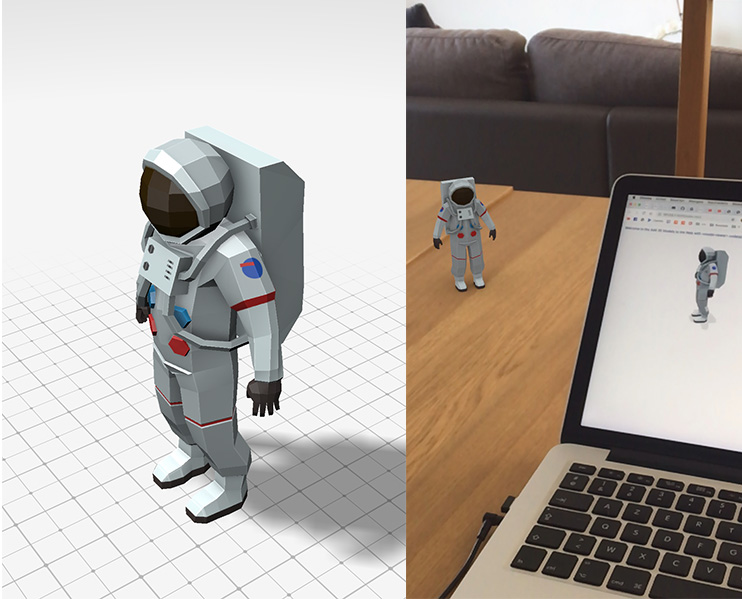
\includegraphics[width=\linewidth]{img/VrAr.jpg}
	\caption{Een illustratie die het verschil tussen VR en AR aanduidt.}
	\label{fig-ar-vr}
\end{figure}

\section{Het gebruik van WebXR}
\label{src:het-gebruik-van-webxr}
De dag van vandaag ondersteunt de Chrome die de meesten van ons kennen nog altijd geen WebXR en moeten er dus enkele stappen gedaan worden alvorens een project die gebruik maakt van de WebXR API kan getest worden. Om zo'n project te testen moet er op het apparaat in kwestie Chrome Canary gedownload worden. Een experimentele browser gemaakt voor designers, ontwikkelaars die telkens de nieuwe snufjes en functionaliteiten los laat zonder veel getest te zijn. In Chrome Canary kunnen er onder de link 'chrome://flags' heel veel functionaliteiten naar uw wens geactiveerd of gedeactiveerd worden. Een daarvan is 'WebXR Device API' en zoals u al verwacht had moet deze geactiveerd worden. 
\textbf{Let op:} indien u een VR-ervaring wilt testen hebt u geen nood aan Chrome Canary maar kan het mogelijk zijn dat uw VR-bril dit reeds ondersteunt.


\subsection{VR}
\label{src:vr}
Om te illustreren hoe VR en AR de WebXR API gebruikt, wordt er in deze sectie eerst uitgelegd hoe u een fictieve wereld kan toevoegen aan uw website. Gebruikers kunnen dan op de website gaan en met behulp van een knop in die fictieve wereld geraken. 

\begin{figure}
	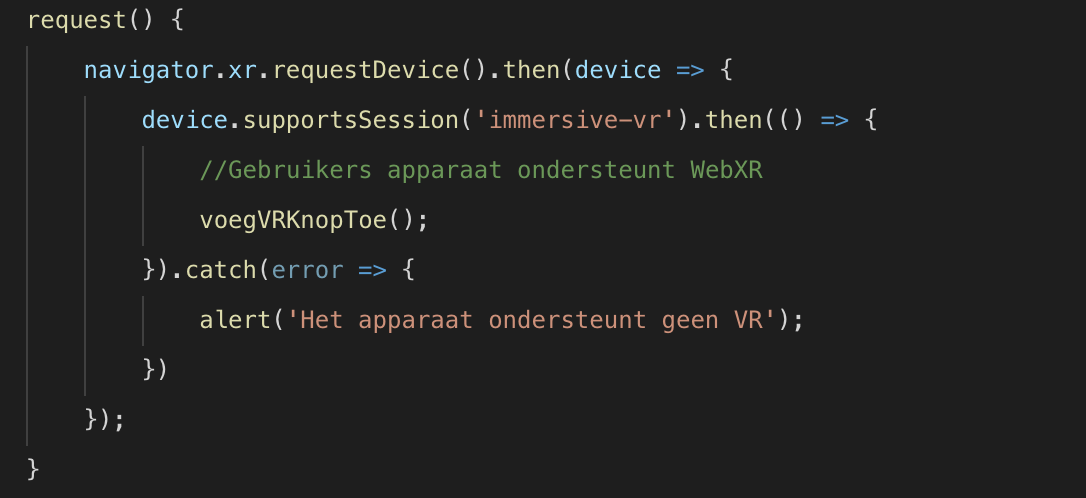
\includegraphics[width=\linewidth]{img/requestVR.png}
	\caption{De code voor te controleren of het apparaat WebXR ondersteunt.}
	\label{fig-requestVR}
\end{figure}

De eerste stap bij het bieden van een VR-ervaring op uw website is om te controleren of het apparaat in kwestie wel degelijk WebXR ondersteunt. Op die manier kan u op uw website iets anders tonen indien dit niet geval is. 
In figuur \ref{fig-requestVR} is de code te zien waarmee dit gecontroleerd wordt. Op regel twee wordt de functie 'navigator.xr.requestDevice()' uitgevoerd. Deze functie controleert of het apparaat in kwestie eender welk XR-apparaat is. Vervolgens wordt er op regel drie gekeken of het apparaat de mode VR ondersteunt. Indien dit het geval is moet gebruiker verwittigd worden dat hij deel kan nemen aan een VR-ervaring. Indien dit niet lukt kan er eender wat gedaan worden om dit op te vangen. Iets anders tonen, de gebruiker melden dat dit niet gaat, etc. 
De volgende stap is om indien de gebruiker op de VR-knop heeft geklikt een WebXR sessie aan te vragen. Deze sessie geeft de website toegang tot alle mogelijkheden van AR en VR op het apparaat. Dat wilt in het geval van een VR-apparaat zeggen dat de website toegang krijgt tot bijvoorbeeld de displays. In figuur \ref{fig-startVR} is te zien hoe op regel drie een sessie wordt aangevraagd met de functie 'requestSession'. Er wordt hierbij exclusieve toegang tot het VR-apparaat gevraagd door te vermelden dat het over een 'immersive-vr' ervaring gaat. Vervolgens moet de website weten hoe hij objecten kan plaatsen in de omgeving ten opzichte van de gebruiker. Hiervoor wordt er op regel vier een frame of reference aangevraagd aan de sessie. Het interessante hierbij is dat er gespecificeerd wordt naar een 'stage' frame of reference, wat er voor zorgt dat het centrum in de fictieve wereld gelijk wordt gezet met de vloer van de gebruiker. Nadien wordt er op regel vijf een 'WebGLLayer' aangemaakt. Dit is een soort van kader waarin alle inhoud van de VR-ervaring in mag getoond worden. In het geval van VR zal deze laag dus ook de hele grootte van de VR-apparaat zijn displays. Ten laatste wordt er op regel zes een animatielus gestart door de functie 'requestAnimationFrame' uit te voeren op de sessie. Deze animatielus ofwel renderlus zal er voor zorgen dat verscheidene keren per seconde de frames gerenderd worden die getoond moeten worden op de displays van het VR-apparaat.

\begin{figure}
	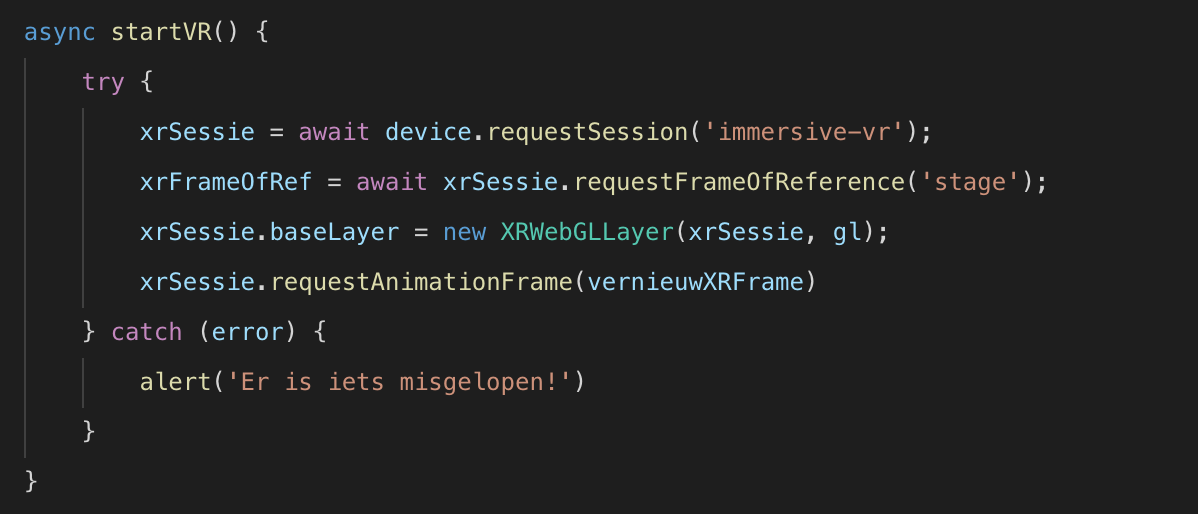
\includegraphics[width=\linewidth]{img/startVR.png}
	\caption{De code om een WebXR sessie te starten voor VR.}
	\label{fig-startVR}
\end{figure}

\subsection{Magic window}
\label{sec:magic-window}
Magic window functionaliteit is ook een leuk extraatje die aan bod komt wanneer het gaat over immersive ervaringen. Het laat gebruikers zonder immersive apparaat toe de ervaringen op een ietwat dezelfde manier te beleven. Magic window zorgt er eigenlijk voor dat er op een 2D website een canvas wordt toegevoegd waarin de immersive inhoud getoond kan worden. Denk maar aan de 360 graden of 3D foto's die u kan zien op uw facebookpagina. Wat dit betekent voor de gebruikers van een smartphone of tablet is dat de wereld zichtbaar vanuit de website zal meedraaien met het apparaat. Indien de gebruiker zich dan rond zijn as draait, zal de fictieve wereld ook meedraaien. Voor computergebruikers kan hetzelfde bereikt worden door met de de muis te slepen in het kader. 

\begin{figure}
	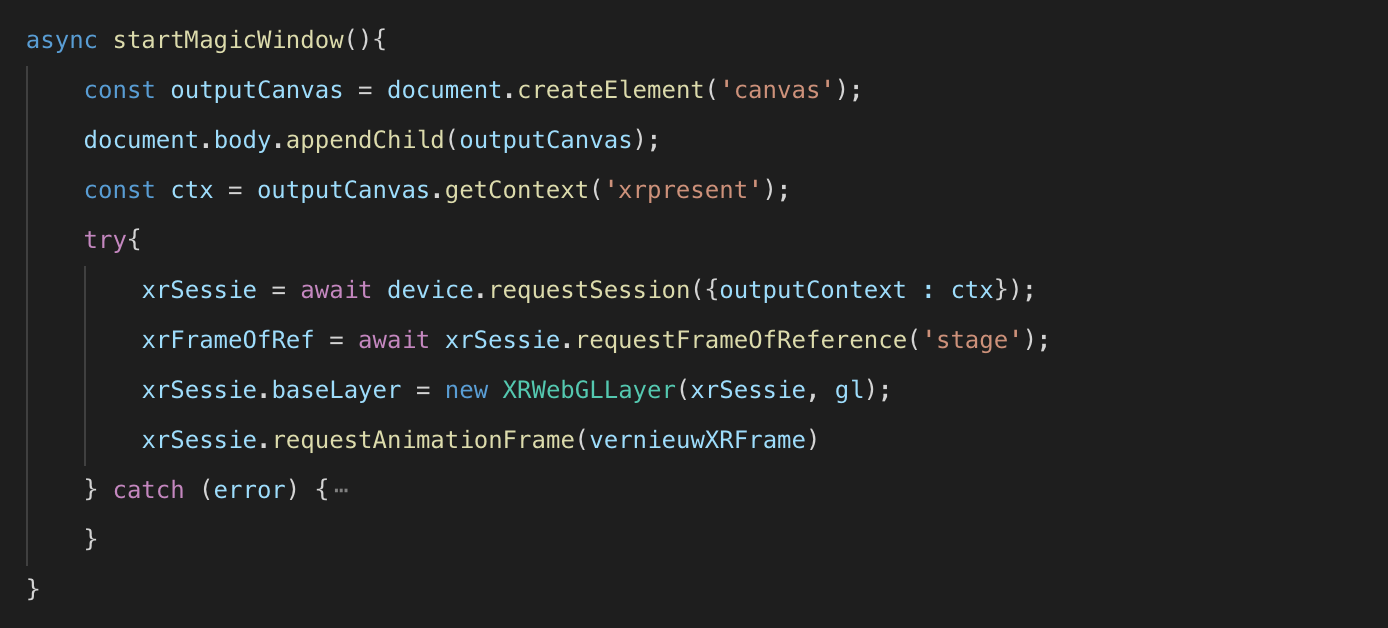
\includegraphics[width=\linewidth]{img/magicWindow.png}
	\caption{De code om een magic window te starten.}
	\label{fig-magic-window}
\end{figure}

Stel nu in voorbeeld van daarnet, dat we wensen om de VR-ervaring niet weer te geven op het VR-apparaat maar in een magic window op de website. Op vlak van code verandert er dan niet zoveel. In figuur \ref{fig-magic-window} zijn de gelijkenissen te zien tussen de code voor VR en de code om een magic window te starten. Op regel twee, drie en vier wordt het canvas aangemaakt en op de website toegevoegd. Vervolgens wordt er op regel zes weer een WebXR sessie aangevraagd. Alleen wordt er hier niet meer exclusieve toegang tot het VR-apparaat gevraagd maar wordt de gerenderde uitvoer, of anders gezegd het zichtbare gedeelte, gelinkt aan de canvas.   


\subsection{AR}
\label{sec:AR}
Zoals eerder vermeld hebben AR en VR veel gelijkenissen. Maar dit is dankzij de WebXR API nu ook op vlak van code. In figuur \ref{fig-start-ar} is heel gelijkaardige code te zien met toen we een magic window wouden maken voor VR op onze website. Echter liggen de 2 grootste verschillen in regel 5 en 7. Waar er voor een VR-ervaring de parameter 'immersive-vr' werd meegegeven, wordt er bij AR nu 'immersive-ar' meegegeven. De achterliggende werking blijf wel hetzelfde in de manier dat er exclusieve toegang wordt gevraagd tot het apparaat zijn display(s). Het ander verschil is dat er voor AR nu een 'eyelevel' frame of reference wordt gespecificeerd. Deze parameter zorgt er voor dat op het moment dat de AR-ervaring start, de huidige positie en oriëntatie wordt gebruikt om de AR-ervaring gelijk mee te zetten. Verder gebruikt AR dezelfde technologie voor het renderen van de de frames voor het display. 

\begin{figure}
	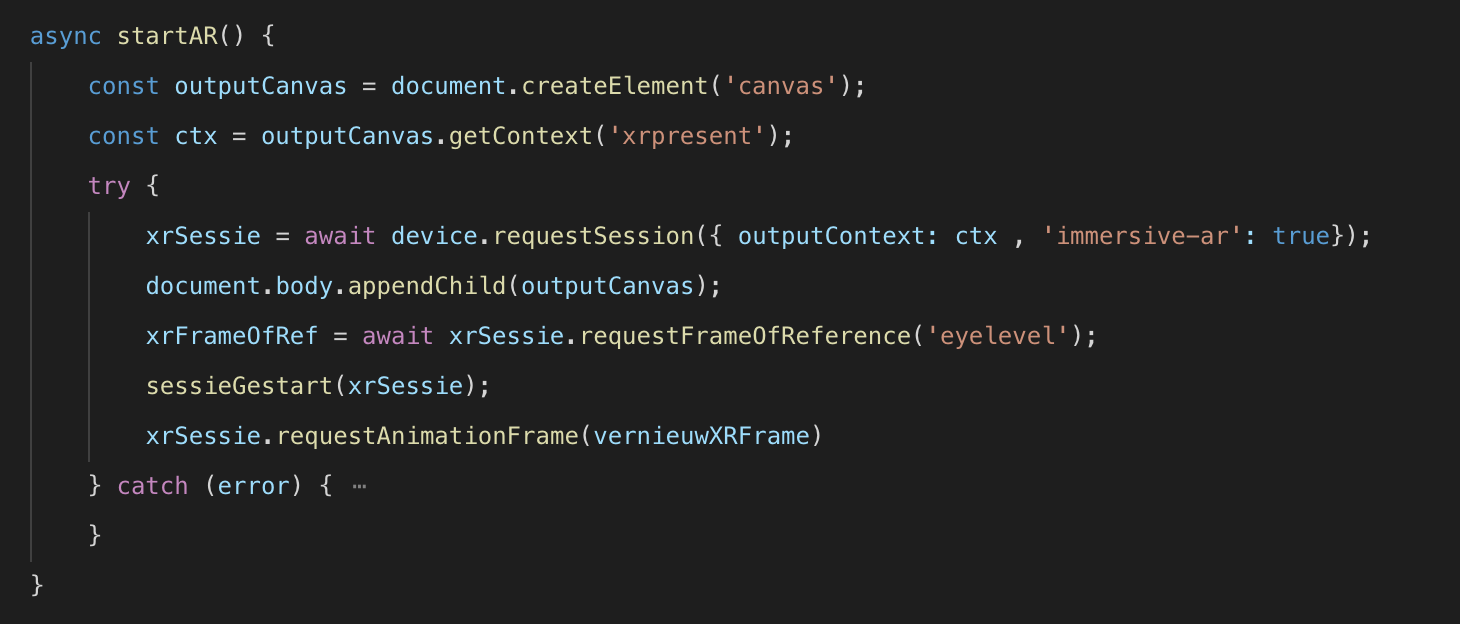
\includegraphics[width=\linewidth]{img/startAR.png}
	\caption{De code om een WebXR sessie te starten voor AR.}
	\label{fig-start-ar}
\end{figure}

\subsection{Hit tests}
\label{src:hit-tests}
Het laatste puntje nodig in dit gehele verhaal om een object te kunnen plaatsen in uw omgeving is de hit test API. Zoals vermeld in sectie \ref{ch:stand-van-zaken} State of the art dienen hit tests om te weten hoe 3D-objecten geplaatst moeten worden in uw omgeving. Het apparaat kan dus in de omgeving andere objecten herkennen zoals tafels, stoelen, ... om zo een besef te verkrijgen van de omgeving.

